% =====================================================================================================
%  ECONOMIC VALUE OF ACTING ON THE MODELS: COST-LOSS ANALYSIS -- paste-in blocks for manuscript.tex
%
%  Answers the referee's request to compare avoided losses with intervention costs and the consequences of
%  false warnings, without a trading simulation. Use these blocks INSTEAD of the LP-backtest blocks of
%  folder 14 (the LP backtest can be kept as an appendix illustration or dropped).
%
%  Setup (once):
%   * copy  paper/generated/*.tex  into a folder  cl/  of the Overleaf project,
%   * copy  figures/cl_*.png       into the project's  figures/  folder,
%   * add   \input{cl/cl_numbers}  to the preamble, and the two entries of cost_loss_refs.bib to updated.bib.
%  After re-running  cost_loss.py, figures.py, paper_tables.py  re-copy both folders; paper_tables.py prints
%  CLAIM OK / CLAIM FAILS for every qualitative statement made below.
% =====================================================================================================


% -----------------------------------------------------------------------------------------------------
% [A] ABSTRACT -- insert after "... with statistically significant gains."
% -----------------------------------------------------------------------------------------------------
In a cost-loss evaluation that charges every warning, false ones included, acting on the early warnings
realises \clHoVa{} of the value of perfect foresight for users who weigh a missed depeg against a hundred
interventions, and the probabilistic forecasts can be used to screen the warnings when interventions are
costly.


% -----------------------------------------------------------------------------------------------------
% [B] HIGHLIGHTS -- add as a fourth item
% -----------------------------------------------------------------------------------------------------
\item A cost-loss analysis quantifies when acting on warnings and forecasts pays off.


% -----------------------------------------------------------------------------------------------------
% [C1] INTRODUCTION -- new paragraph after the paragraph ending
%      "... while the forecaster characterizes its direction and severity."
% -----------------------------------------------------------------------------------------------------
Detection rates and scoring rules do not by themselves show that acting on the models is worthwhile. We
therefore evaluate them in the cost-loss framework of forecast verification
\citep{Murphy1977,Richardson2000}, in which a user pays a cost for every protective action, including those
prompted by false warnings, and incurs a larger loss for every event that was not anticipated. The framework
requires no assumption about the user's position or trading strategy beyond the ratio of the two costs, and
it reports the value of a warning or forecasting system for every such ratio. Acting on the classifier's
warnings pays for any user whose loss from a missed event exceeds the cost of about \clHoPays{}
interventions over the holdout, and of about \clCvPays{} in cross-validation. The forecaster's probabilities
add value where interventions are relatively costly, by screening the warnings.

% [C2] INTRODUCTION -- replace the roadmap sentence
%      "Section \ref{sec:results} reports the empirical results, and Section \ref{sec:conclusion} concludes."
Section~\ref{sec:results} reports the empirical results, including the economic value of acting on the
models in Section~\ref{sec:cl_results}, and Section~\ref{sec:conclusion} concludes.


% -----------------------------------------------------------------------------------------------------
% [D] METHODOLOGY -- new subsection at the end of Section 3, immediately before
%     "\section{Results}\label{sec:results}"
% -----------------------------------------------------------------------------------------------------
\subsection{Economic value of acting on the models}\label{sec:cl_method}

We measure the value of acting on the models with the cost-loss model of forecast verification
\citep{Murphy1977,Richardson2000}. A user exposed to a depeg of the pool can take a protective action, such
as reducing or hedging a position, at a cost $c$, and incurs a loss $L>c$ if a depeg occurs while
unprotected. The user is characterised only by the ratio $c/L\in(0,1)$, and we report value over the whole
range of ratios rather than for an assumed user.

\paragraph{Early warnings.} Each alert episode is a warning that triggers one protective action, so false
warnings cost $c$. An eligible event is anticipated if an alert episode begins 2 to 24 hours before its first
breach, the timeliness criterion of Eq.~\eqref{eq:timely_event_recall}; an event that is not anticipated
costs $L$. With $D$ anticipated events out of $N$ and $W$ warnings, the expense of acting on the warnings is
$cW+L(N-D)$, against $LN$ for never acting and $cN$ for a perfect warning system. The relative economic value,
the share of the saving of a perfect system that the warnings realise, is
\begin{equation}
V(c/L)=\frac{LN-\left[cW+L(N-D)\right]}{LN-cN}=\frac{D-(c/L)\,W}{N\,(1-c/L)}.
\label{eq:cl_value}
\end{equation}
$V$ is positive when $c/L<D/W$, the number of anticipated events per warning, and tends to the event recall
$D/N$ as $c/L\to0$. The break-even ratio $D/W$ therefore summarises the trade-off between avoided losses and
the cost of false warnings: acting on the warnings pays for any user whose loss from a missed event exceeds the
cost of $W/D$ interventions. We compute $V$ for every candidate classifier in cross-validation and for the
selected specification over the holdout. As a model-free benchmark, a \emph{price precursor} warns when
$|d_t|$ reaches 8, 10 or 12\,bp, with the same 12-hour quiet reset; it uses only the current price.

\paragraph{Probabilistic forecasts.} For the forecaster, a user decides at each hour whether to protect
against $|d_{t+h}|\geq\theta$ and acts when the forecast exceedance probability exceeds $c/L$, the optimal
rule for a calibrated forecast. The relative economic value compares the expense of this rule with the
better of always and never protecting and with perfect information \citep{Richardson2000}. We evaluate
$h\in\{6,12,24\}$ hours and $\theta\in\{10,15\}$\,bp for all forecasters over the holdout.

\paragraph{Joint use.} The two models answer different questions: the classifier signals that an event may
be approaching, and the forecaster quantifies how likely a breach is. In the joint rule, a user acts on a
classifier warning only if the forecaster's probability of a 15\,bp breach within the next 2 to 24 hours,
computed as the largest marginal exceedance probability over these horizons, exceeds $c/L$. The rule needs
no tuning: each user screens the warnings at their own cost-loss ratio. We compare it with acting on every
warning and with the forecaster alone, which acts whenever the same probability exceeds $c/L$. Because the
neural forecasts cover only the holdout, the joint evaluation is restricted to that period.


% -----------------------------------------------------------------------------------------------------
% [E] RESULTS -- new subsection at the end of Section 4, after Figure \ref{fig:stress_calm_ablation} and
%     immediately before "\section{Conclusion and Perspectives}"
% -----------------------------------------------------------------------------------------------------
\subsection{Economic value of acting on the models}\label{sec:cl_results}

\paragraph{Early warnings.} Table~\ref{tab:cl_classifier} and Figure~\ref{fig:cl_classifier} report the
value of acting on the warnings. Over the holdout, the selected policy anticipates all \clHoN{} events with
\clHoW{} warnings, so acting on them pays for any user whose loss from a missed event exceeds the cost of
\clHoPays{} interventions. For a user who weighs a missed event against a hundred interventions
($c/L=0.01$), the warnings realise \clHoVa{} of the value of perfect foresight, and \clHoVb{} at $c/L=0.05$.
In cross-validation the policy anticipates \clCvD{} of \clCvN{} events with \clCvW{} warnings, which pays
for missed-event losses above \clCvPays{} interventions. It dominates every other model family at every
cost-loss ratio: the best alternative, \clCvOther, anticipates \clCvOtherD{} events, for a value of
\clCvOtherVa{} at $c/L=0.01$ against \clCvVa.

\input{cl/tab_cl_classifier}

\begin{figure}[pos=!htbp,align=\centering]
    \centering
    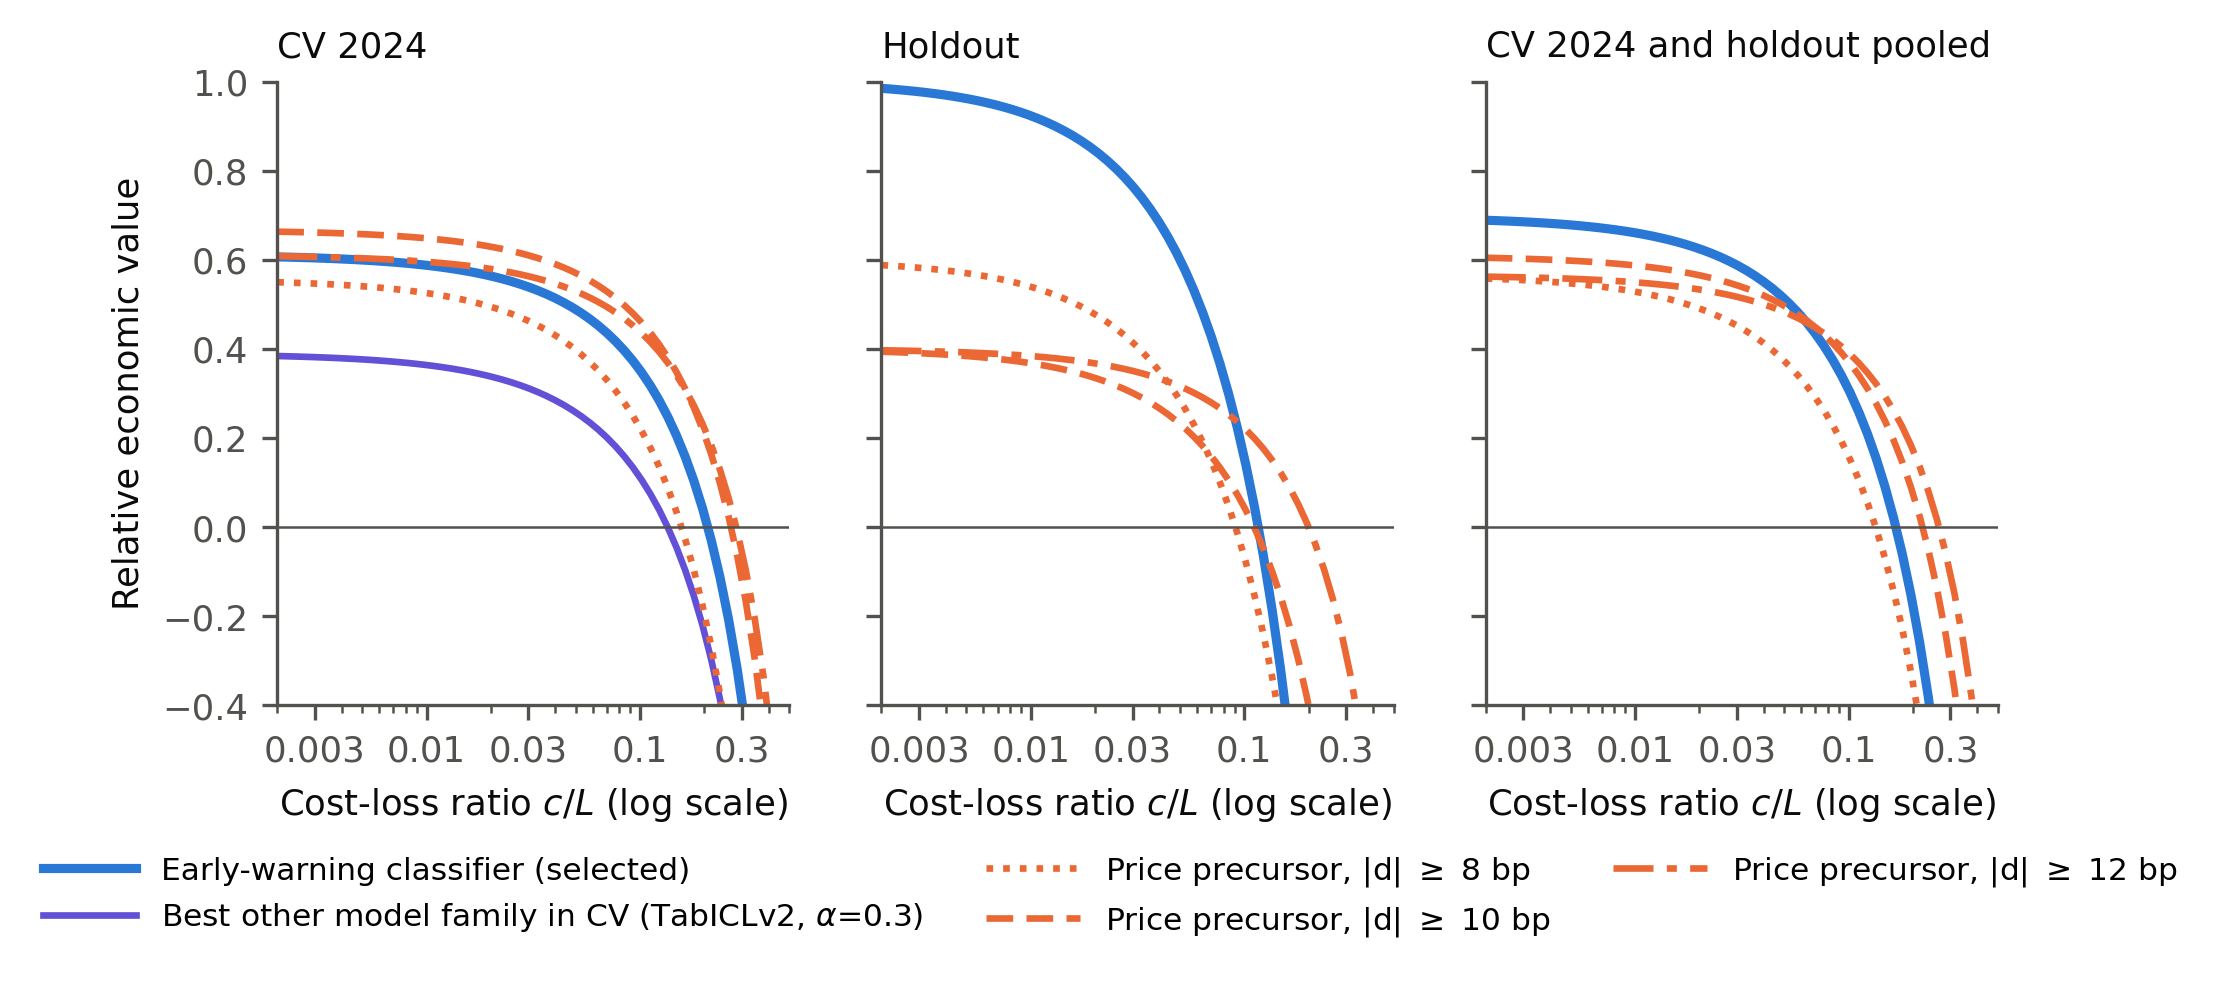
\includegraphics[width=\linewidth]{figures/cl_classifier_value.png}
    \caption{Relative economic value of acting on early warnings as a function of the cost-loss ratio $c/L$:
    the share of the saving of a perfect warning system realised by the rule. Values below zero mean that the
    cost of the warnings exceeds the losses they avoid.
    \href{https://github.com/QuantLet/onchain-insights/tree/main/15.\%20Cost-loss\%20analysis}{\includegraphics[height=0.6\baselineskip]{figures/Quantlet LOGO.png}}}
    \label{fig:cl_classifier}
\end{figure}

The price precursors are a demanding benchmark. In cross-validation, warning when $|d_t|$ reaches 10\,bp
anticipates \clCvPreTenD{} events with \clCvPreTenW{} warnings and therefore has higher value than the
classifier at every ratio. Over the holdout, the precursors anticipate at most \clHoPreMaxD{} of the
\clHoN{} events, and their value at $c/L=0.01$ is at most \clHoPreBestVa. Pooling both samples, the
classifier anticipates \clPoD{} of \clPoN{} events with \clPoW{} warnings, against \clPoTenD{} events with
\clPoTenW{} warnings for the 10\,bp precursor. The classifier is therefore the better rule for users whose
loss from a missed event exceeds the cost of about \clPoCrossTenInv{} interventions ($c/L<\clPoCrossTen$),
and the precursor for users with cheaper misses. Over the holdout, the classifier anticipates
\clHoOnlyClassifierTen{} events that the 10\,bp precursor misses, so price proximity to the threshold does not
by itself explain its warnings.

\paragraph{Probabilistic forecasts.} Figure~\ref{fig:cl_forecaster} and Table~\ref{tab:cl_forecaster} report
the value of acting on the forecast exceedance probabilities. Our model has the highest Brier skill in
\clFcBestBSSCells{} of the \clFcCells{} combinations of horizon and threshold. Its advantage is clearest for
15\,bp moves when protection is relatively costly: at a 12-hour horizon its value is \clFcTwelveFifteenVc{}
at $c/L=0.1$ and \clFcTwelveFifteenVd{} at $c/L=0.2$, the highest of all forecasters, while GARCH has
negative value (\clFcTwelveFifteenGarchVc) and TimeXer almost none (\clFcTwelveFifteenTimeXerVc). Acting on
those probabilities requires well-calibrated tails, because a user with a high cost-loss ratio acts only when
the forecast probability is high. For users who protect at the first sign of risk ($c/L\leq0.02$), the
rolling empirical benchmark, whose tails are wider, has slightly higher value. At a 24-hour horizon no
forecaster has value for 15\,bp moves at $c/L=0.1$: exceedances at a fixed horizon that far ahead are too
rare to act on, which is the role of the early-warning classifier.

\begin{figure}[pos=!htbp,align=\centering]
    \centering
    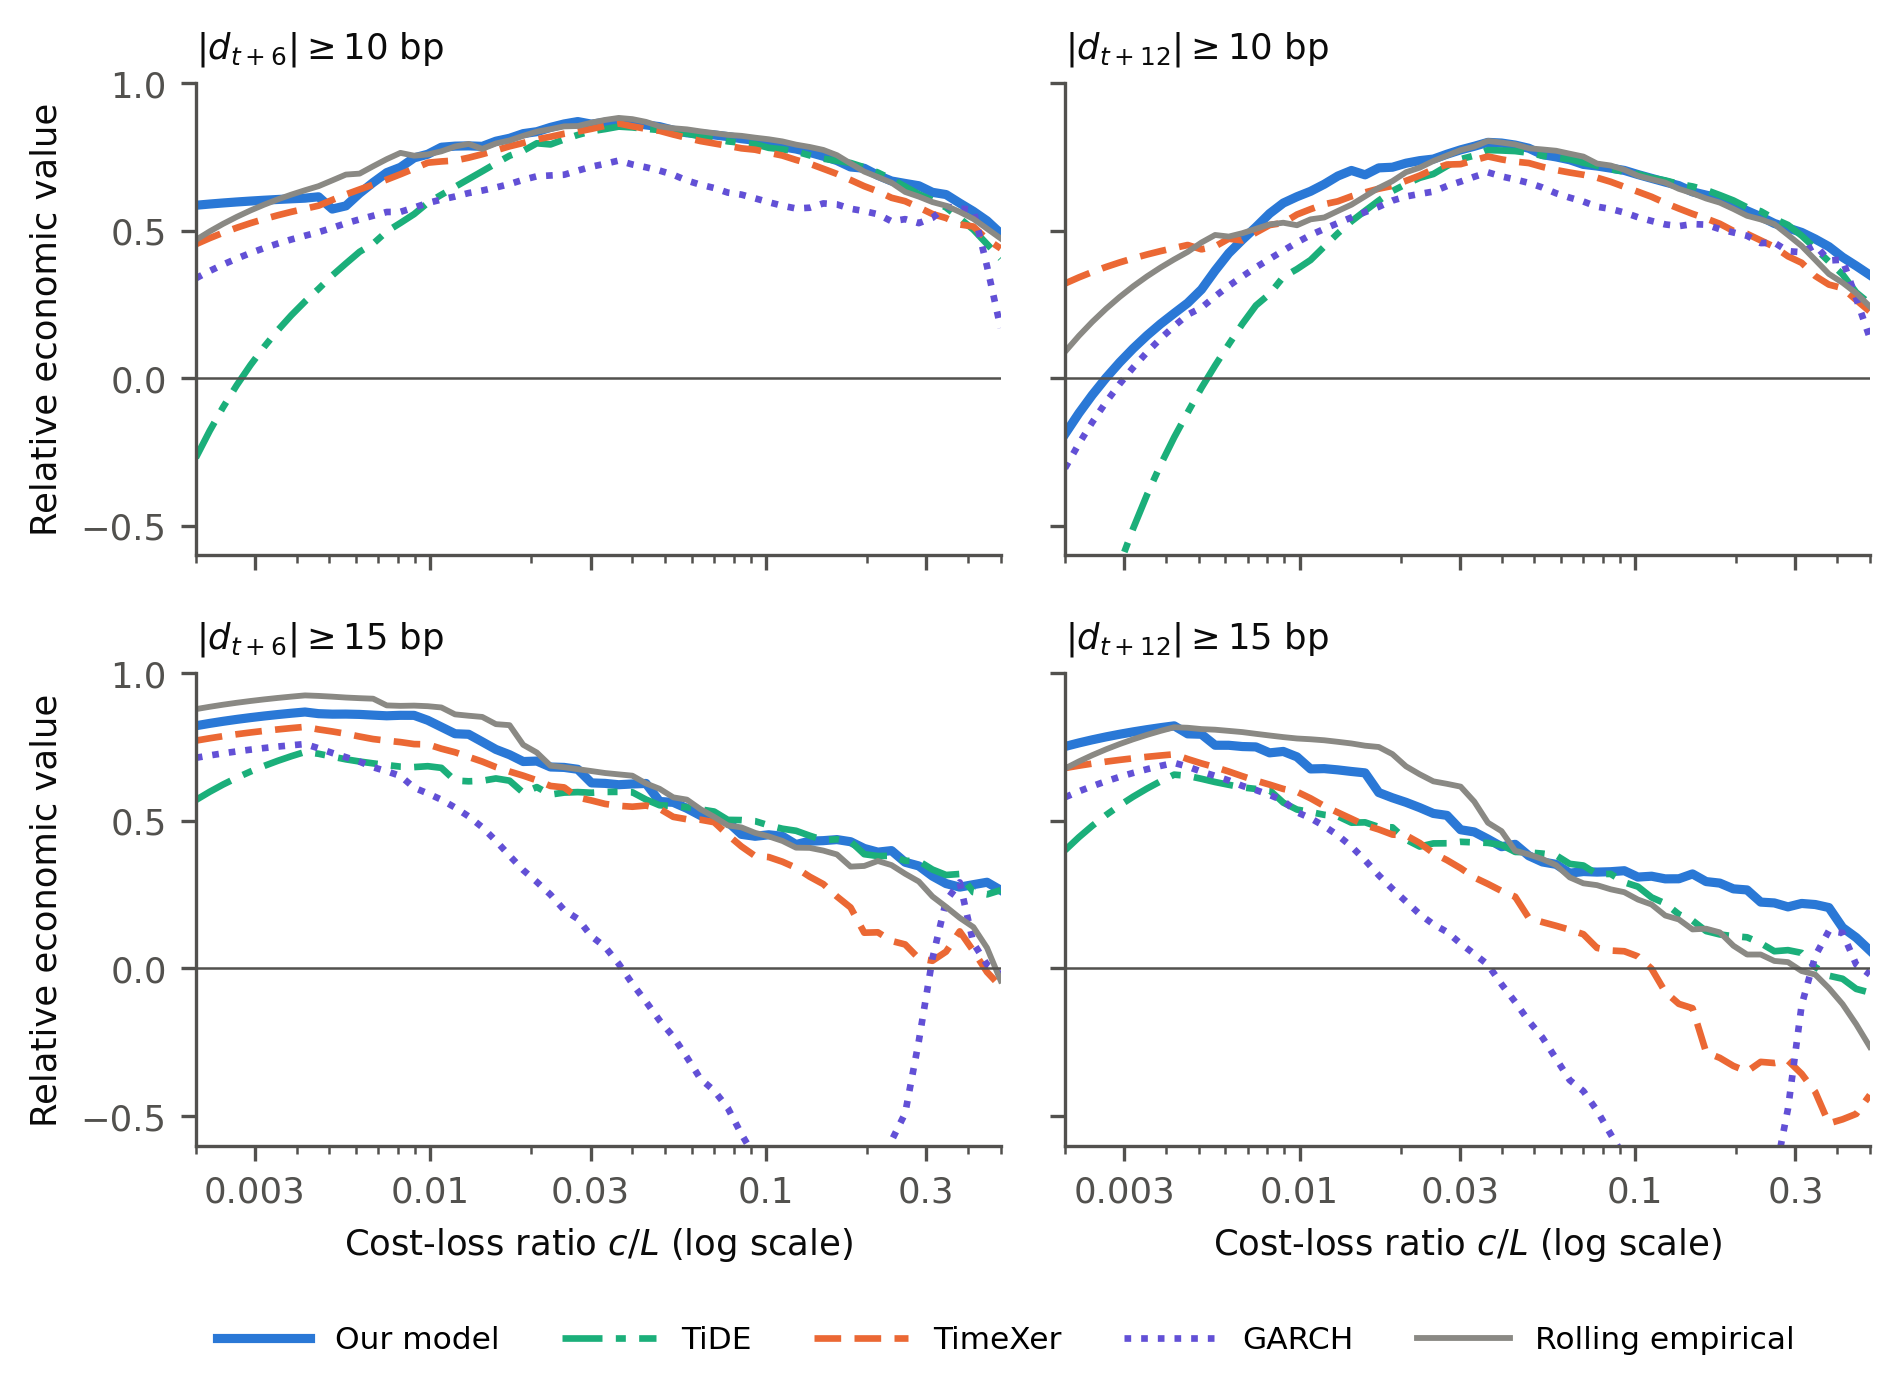
\includegraphics[width=\linewidth]{figures/cl_forecaster_value.png}
    \caption{Relative economic value of protecting against $|d_{t+h}|\geq\theta$ whenever the forecast
    exceedance probability exceeds the cost-loss ratio $c/L$, over the holdout.
    \href{https://github.com/QuantLet/onchain-insights/tree/main/15.\%20Cost-loss\%20analysis}{\includegraphics[height=0.6\baselineskip]{figures/Quantlet LOGO.png}}}
    \label{fig:cl_forecaster}
\end{figure}

\paragraph{Joint use.} The forecaster helps to separate true from false warnings. At the start of the
classifier's \clJointTimely{} timely and \clJointFalse{} false warnings over the holdout, the forecast breach
probability ranks timely above false warnings with an AUC of \clJointAUC{} (Figure~\ref{fig:cl_joint}, right).
The two models therefore serve different users (Figure~\ref{fig:cl_joint}, left; Table~\ref{tab:cl_joint}).
When missed events are costly relative to interventions, acting on every warning is best: at $c/L=0.01$ its
value is \clJointClVa, against \clJointVa{} for the joint rule, which discards some timely warnings. When
interventions are more costly, screening the warnings with the forecaster is better: from $c/L\approx
\clJointCross$, a missed event worth fewer than about \clJointCrossInv{} interventions, the joint rule has
the higher value, \clJointVc{} against \clJointClVc{} at $c/L=0.1$. The classifier determines when to
consider acting, and the forecaster determines whether acting is worth its cost.

\input{cl/tab_cl_joint}

\begin{figure}[pos=!htbp,align=\centering]
    \centering
    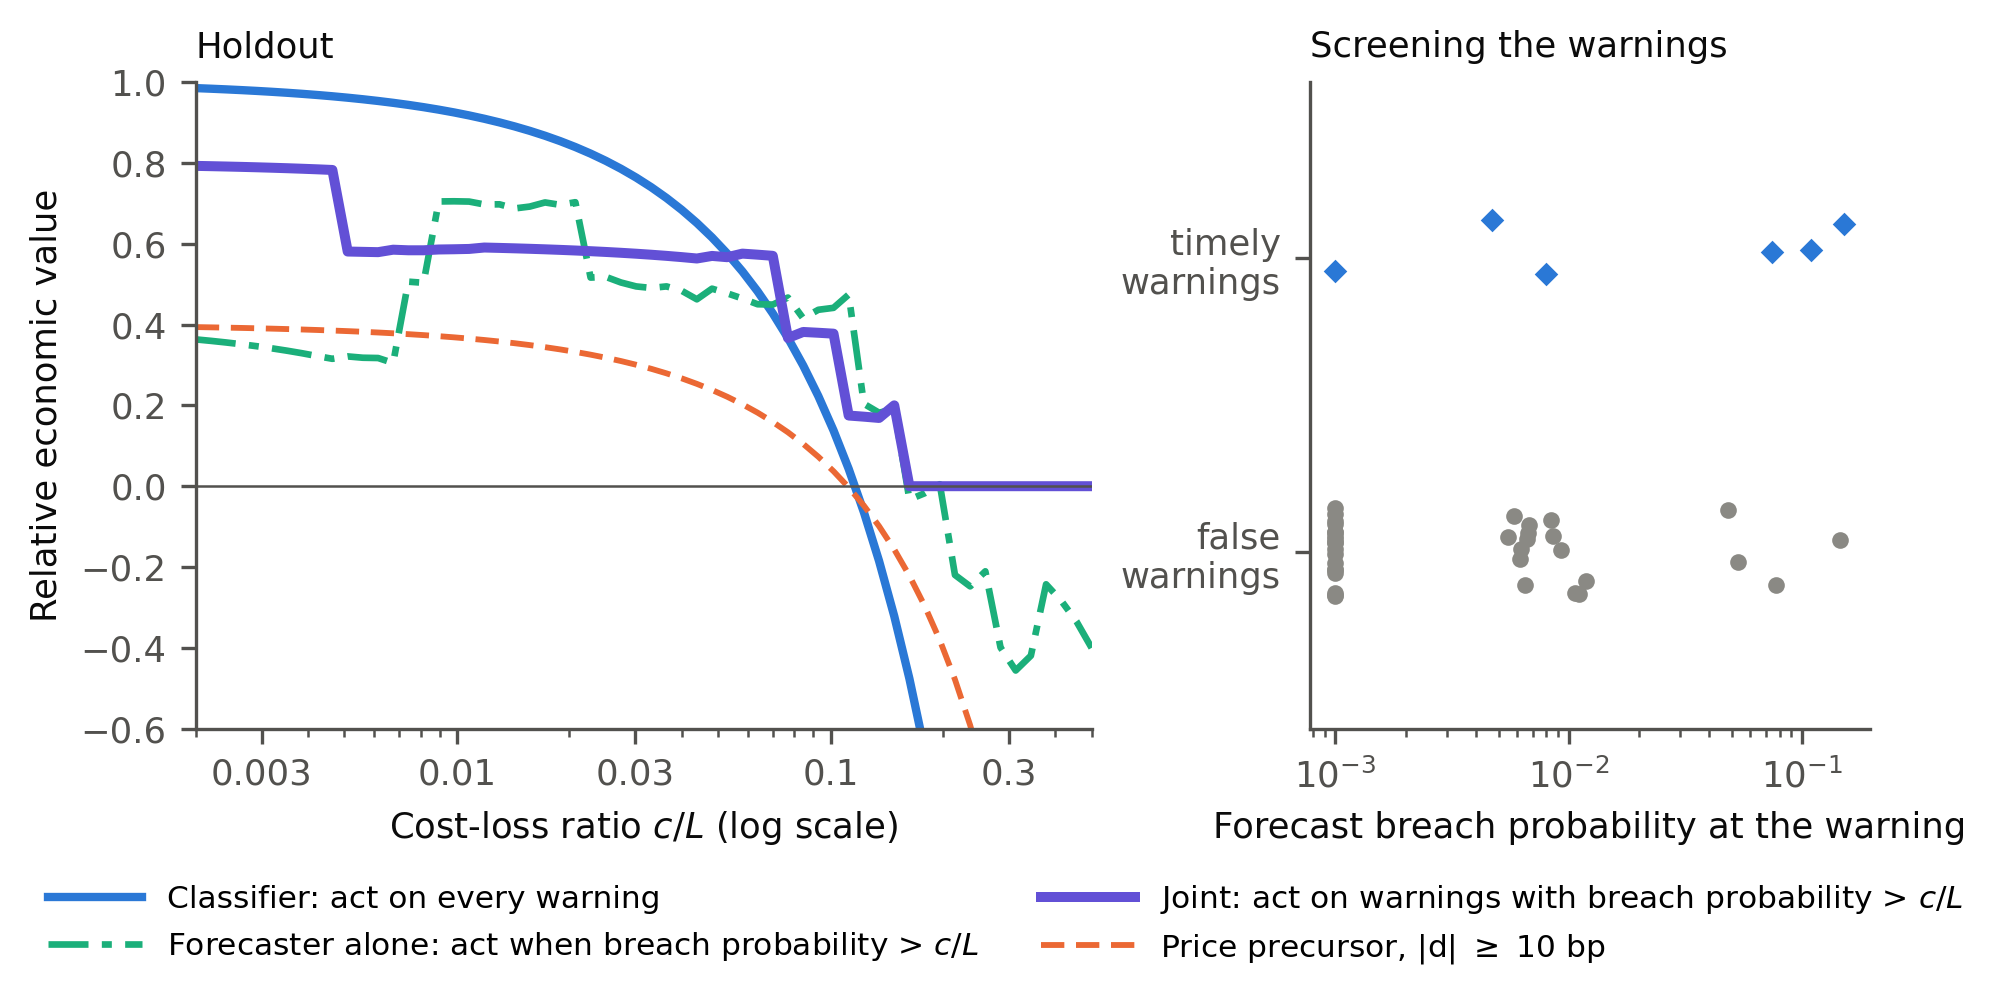
\includegraphics[width=\linewidth]{figures/cl_joint_value.png}
    \caption{Joint use of the two models over the holdout. Left: relative economic value of acting on every
    classifier warning, on the forecaster alone, and on the warnings whose forecast breach probability exceeds
    the user's cost-loss ratio. Right: forecast probability of a 15\,bp breach in the next 2 to 24 hours at the
    start of each warning; probabilities below 0.001 are shown at 0.001.
    \href{https://github.com/QuantLet/onchain-insights/tree/main/15.\%20Cost-loss\%20analysis}{\includegraphics[height=0.6\baselineskip]{figures/Quantlet LOGO.png}}}
    \label{fig:cl_joint}
\end{figure}

\paragraph{Limitations.} The cost-loss model reduces each user to one ratio and treats all events as equally
costly; with \clHoN{} holdout and \clCvN{} cross-validation events, the comparisons rest on few events. The
price-precursor thresholds were fixed in advance at 8, 10 and 12\,bp rather than tuned, and all three are
reported. The forecast breach probability is a lower bound on the probability of a breach at some point in
the window, which makes the joint rule conservative.


% -----------------------------------------------------------------------------------------------------
% [F] CONCLUSION -- new paragraph after the second paragraph (ending
%      "... potential severity of prospective pool-price deviations.")
% -----------------------------------------------------------------------------------------------------
A cost-loss analysis quantifies the economic value of acting on the framework, counting the cost of false
warnings. Acting on the early warnings pays for any user whose loss from a missed depeg exceeds the cost of
about \clHoPays{} interventions over the holdout and \clCvPays{} in cross-validation, and realises
\clHoVa{} of the value of perfect foresight for users who weigh a missed depeg against a hundred
interventions. A simple price precursor is competitive in cross-validation but anticipates far fewer
held-out events, so the classifier is the better rule for users with costly misses. The forecaster's
probabilities have the most value where protection is relatively costly, and screening the warnings with
them extends the framework's value to those users: the classifier signals when to consider acting, the
forecaster whether acting is worth its cost.


% -----------------------------------------------------------------------------------------------------
% [G] APPENDIX -- new section, e.g. before "\section{Data Appendix}"
% -----------------------------------------------------------------------------------------------------
\section{Cost-loss analysis: additional results}\label{sec:cl_appendix}

Table~\ref{tab:cl_candidates} reports the economic value of acting on the warnings of every candidate
classifier in cross-validation, and Table~\ref{tab:cl_forecaster} the value of the forecast exceedance
probabilities for all horizons, thresholds and forecasters.

\input{cl/tab_cl_candidates}

\input{cl/tab_cl_forecaster}
